\documentclass[hidelinks,12pt]{article}

\usepackage{amsmath}    % need for subequations
\usepackage{graphicx}   % need for figures
\usepackage{verbatim}   % useful for program listings
\usepackage{color}      % use if color is used in text
\usepackage{subfigure}  % use for side-by-side figures
\usepackage{hyperref}   % use for hypertext links, including those to external documents and URLs

\usepackage[numbered]{matlab-prettifier} % including matlab w/ syntax highlighting
\usepackage[T1]{fontenc} % prettier matlab font
\lstMakeShortInline[style=Matlab-editor]| % matlab inline escape character

\usepackage[
top    = 2.75cm,
bottom = 2.50cm,
left   = 3.00cm,
right  = 2.50cm]{geometry}

\graphicspath{ {./Figures/} }

% don't need the following. simply use defaults
\setlength{\baselineskip}{16.0pt}    % 16 pt usual spacing between lines



\begin{document}
\pagenumbering{gobble}
\begin{center}
  {\huge Homework 5}\\
  \vspace{10px}
  
\includegraphics{Logo} \\
  Date of Submission:\\
  February 25, 2019\\
  \vspace{30px}
  \rule{300px}{0.5px} \\
  Thorne Wolfenbarger \\
  \href{mailto:wolfent1@my.erau.edu}{wolfent1@my.erau.edu} \\
  \vspace{30px}
  Submitted to: \\
  Professor Kaela Martin \\
  College of Engineering \\
  \vspace{40px}
  In Partial Fulfillment \\
  of the Requirements of \\
  \vspace{10px}
  AE 313 \\
  Space Mechanics \\
  Spring, 2019 \\
\end{center}

\pagenumbering{arabic}
\begin{center}
\large AE 313 Homework 5
\end{center}
\flushleft
1. Find $e, E_0, (t_0-t_p).$\\
  ~~$e = 0.453$\\
  ~~$E_0 = -1.8076$\\
  ~~$(t_0-t_p) = -3.4481 \cdot 10^3$\\
\vspace{5px}
2. Write $\vec{v}$ in terms of radial-transverse vectors $(\hat{r}, \hat{\theta}, \hat{h}).$\\
  ~~$\vec{v} = -1.0231 \hat{r} + 2.0714 \hat{\theta}~km/s$\\
\vspace{5px}
3. Using Lagrange coefficients, write the new velocity $(\vec{v}_1)$ in terms of inertial unit vectors $(\hat{x}, \hat{y}, \hat{z})$ and radial-tangential coordinates $(\hat{r}, \hat{\theta}, \hat{h})$\\
  ~~$\vec{v}_1 = 0.5869 \hat{x} - 0.2144 \hat{y} - 1.4488 \hat{z}~km/s$\\
  ~~$\vec{v}_1 = -0.0302 \hat{r} + 1.5775 \hat{\theta}~km/s$\\
\vspace{5px}
4. Write the new position and velocity $(\vec{r}_1, \vec{v}_1)$ in terms of perifocal coordinates $(\hat{e}, \hat{p}, \hat{h})$.\\
  ~~$\vec{r}_1 = (-9.4141 \hat{e} - 0.2174 \hat{p}) \cdot 10^3~km/s$\\
  ~~$\vec{v}_1 = 0.0666 \hat{e} - 1.5764 \hat{p}~km/s$\\
\vspace{5px}
5. Determine the inclination, longitude of the ascending node, and the argument of periapsis of MAVEN's orbit.\\
~~$i = 1.3077~rad = 74.9266^\circ$\\
Inclination is only defined from $0^\circ$ to $90^\circ$ so it is positive.\\
~~$\Omega = 0.3243~rad = 18.5792^\circ$\\
$\Omega$ is solved for by two equations in the MATLAB code.\\
~~$\omega = 1.0691~rad = 61.2563^\circ$\\
$\omega$ does not need a quadrant check. The underlying $\theta$ has its value as solved by two equations in the MATLAB code.\\
\vspace{5px}
6. Set-up a Mars centered scenario. Propagate the spacecraft for 12 hours. State $i, \Omega, \omega$ and $\vec{r}_1, \vec{v}_1$ in the inertial coordinates $\hat{x}, \hat{y}, \hat{z}$ from GMAT. Are they close to your calculated values? Note you should have position errors of less than 1 km and velocity errors of 0.3 m/s.\\
\begin{figure}[!htb]
  \center
  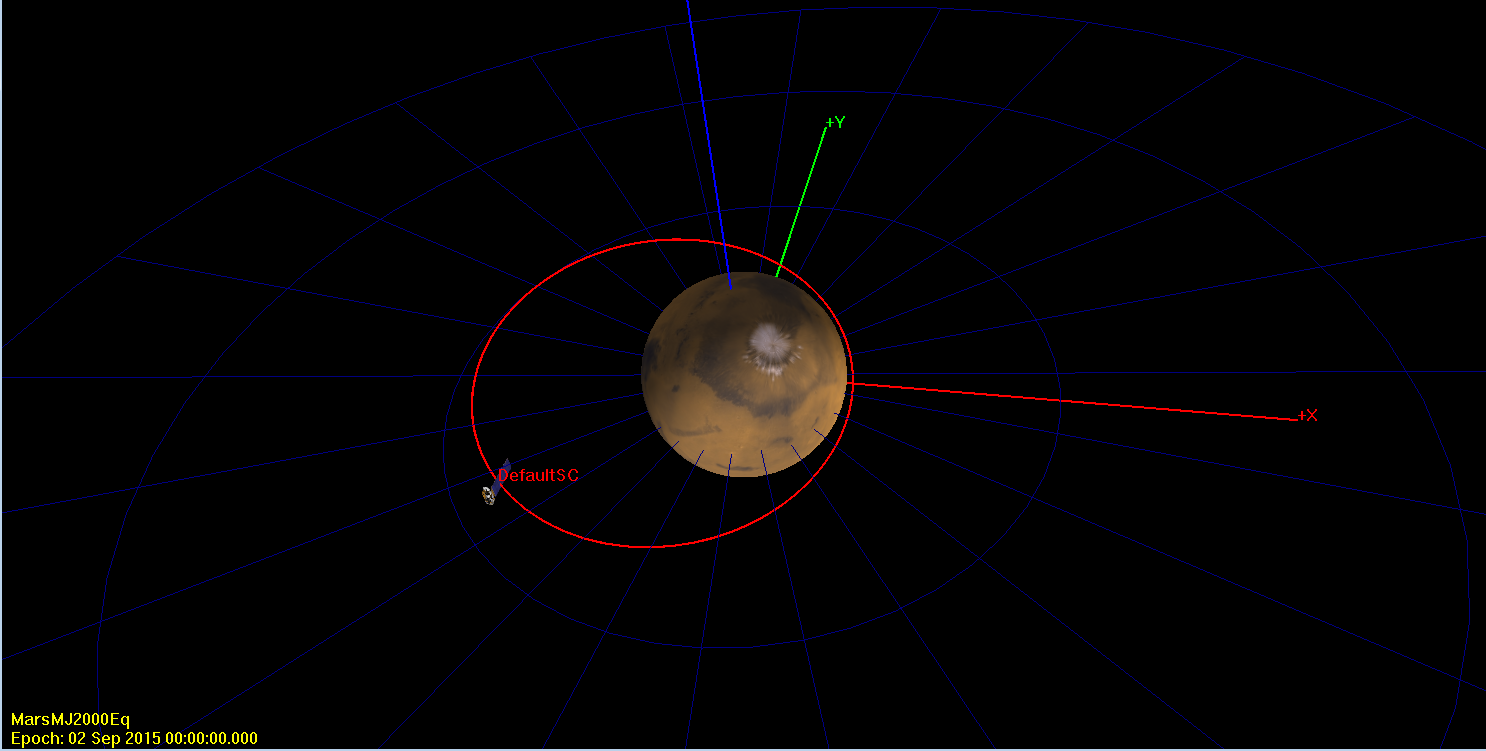
\includegraphics[scale=0.6]{HW5}
  \caption{Martian Orbit}
  \label{}
\end{figure}
\newpage
~From GMAT\\
~~$\vec{r}_1 = (-8.3118 \hat{x} - 3.5461 \hat{y} -2.6476 \hat{z}) \cdot 10^3~km$\\
~~$\vec{v}_1 = 0.5872 \hat{x} -0.2142 \hat{y} -1.4487 \hat{z}~km/s$\\
~From Calculations\\
~~$\vec{r}_1 = (-8.3123 \hat{x} - 3.5460 \hat{y} -2.6466 \hat{z}) \cdot 10^3~km$\\
~~$\vec{v}_1 = 0.5869 \hat{x} -0.2144 \hat{y} -1.4488 \hat{z}~km/s$\\
These values are within the acceptable error.\\
\vspace{5px}
7. If you were planning this trajectory, would you be worried about the lifetime of the spacecraft? Why or why not? What if the trajectory had the same altitude above Earth as it does above Mars?\\
~~I would be worried about the lifetime of the spacecraft. Since the MAVEN is designed to perform atmospheric research it would encounter atmospheric drag. This drag would reduce the lifetime of the space craft by decaying the orbit and wearing down the spaceceraft.\\
If it was at the same altitude above the earth as it is above mars it would be 3545.94 km above the 6390.1 km reach of Earth's atmosphere. More importantly, it would be inside the 6378.1 km radius of Earth at periapsis. This implies that the spacecraft would impact with Earth.

\newpage
HW5.m
\begin{lstlisting}[frame=lines,style=Matlab-editor,basicstyle = \mlttfamily]
clc; clear all; close all

%constants
MU = 42828;

% Problem 1
vr = [-2089.6 -2515.7 -6382.0];
vv = [2.1744 0.76911 0.13452];

r = norm(vr)
v = norm(vv)

vh = cross(vr, vv);
h = norm(vh);

syms a
energy_eqn = v^2/2 - MU/r == -MU/(2*a)
energy = v^2/2 - MU/r
a = double(solve(energy_eqn, a))

syms e
h_eqn = h == sqrt(MU*a*(1-e^2))
e = double(solve(h_eqn,e))
e = max(e)

syms E
E_eqn = r == a*(1-e*cos(E));
E = double(solve(E_eqn,E));
E = -min(E) %Because it is descending.

syms time_since_p
time_since_p_eqn = sqrt(MU/a^3)*time_since_p == E - e*sin(E);
time_since_p = double(solve(time_since_p_eqn,time_since_p))

% Problem 2
p = h^2/MU;
true_a = -acos(p/(r*e) - 1/e)
vv_rt = [h*e/p*sin(true_a) h/r 0] % answer

% Problem 3
E1 = E;
t1 = time_since_p;
vr1 = vr;
vv1 = vv;
r1 = r;
v1 = v;
t2 = time_since_p + 12*60*60;
n = sqrt(MU/a^3);
M = n*t2;
E2 = fzero(@(x) x-e*sin(x)-M, 0);
f = 1 - a/r*(1-cos(E2-E1));
g = (t2 - t1) - sqrt(a^3/MU)*(E2 - E1 - sin(E2 - E1));

vr2 = f*vr + g*vv;
r2 = norm(vr2);
fdot = -sqrt(MU*a)/(r2*r1)*sin(E2-E1);
gdot = 1 - a/r2*(1-cos(E2-E1));

vv2 = fdot*vr1 + gdot*vv1 % intertial unit vectors

true_a2 = -acos(p/(r2*e) - 1/e)

vv2_rt = [h*e/p*sin(true_a2) h/r2 0] % radial-tangential

% Problem 4
vr2_peri = [r2*cos(true_a2) r2*sin(true_a2) 0]
vv2_peri = sqrt(MU/p)*[-sin(true_a2) e+cos(true_a2) 0]

% Problem 5

% find i theta omega
syms inc
h_hat = cross(vr2, vv2)/norm(cross(vr2, vv2))
inc_eqn = cos(inc) == dot(h_hat, [0 0 1])
inc = double(solve(inc_eqn,inc))
inc = max(inc)

syms RAAN
RAAN_eqn_1 = sin(RAAN)*sin(inc) == dot(h_hat, [1 0 0])
RAAN_eqn_2 = -cos(RAAN)*sin(inc) == dot(h_hat, [0 1 0])
RAAN1 = double(solve(RAAN_eqn_1));
RAAN2 = double(solve(RAAN_eqn_2));
RAAN = min(RAAN1)*180/pi

syms arg_peri
r1_hat = vr1/norm(vr1)
theta_hat = cross(r1_hat, h_hat)/norm(cross(r1_hat, h_hat))
syms theta
theta_eqn_1 = sin(inc) * sin(theta) == dot(r1_hat, [0 0 1])
theta_eqn_2 = sin(inc) * cos(theta) == dot(theta_hat, [0 0 1])
theta1 = double(solve(theta_eqn_1, theta))
theta2 = double(solve(theta_eqn_2, theta))
theta = intersect(theta1, theta2)
arg_peri_eqn = arg_peri == theta - true_a
arg_peri = double(solve(arg_peri_eqn, arg_peri))
\end{lstlisting}

\end{document}
